%%%%%%%%%%%%%%%%%%%%%%%%%%%%%%%%%%%%%%%%%
% Journal Article
% LaTeX Template
% Version 1.4 (15/5/16)
%
% This template has been downloaded from:
% http://www.LaTeXTemplates.com
%
% Original author:
% Frits Wenneker (http://www.howtotex.com) with extensive modifications by
% Vel (vel@LaTeXTemplates.com)
%
% License:
% CC BY-NC-SA 3.0 (http://creativecommons.org/licenses/by-nc-sa/3.0/)
%
%%%%%%%%%%%%%%%%%%%%%%%%%%%%%%%%%%%%%%%%%

%----------------------------------------------------------------------------------------
%	PACKAGES AND OTHER DOCUMENT CONFIGURATIONS
%----------------------------------------------------------------------------------------

\documentclass[twoside,twocolumn]{article}

\usepackage{blindtext} % Package to generate dummy text throughout this template

\usepackage[sc]{mathpazo} % Use the Palatino font
\usepackage[T1]{fontenc} % Use 8-bit encoding that has 256 glyphs
\linespread{1.05} % Line spacing - Palatino needs more space between lines
\usepackage{microtype} % Slightly tweak font spacing for aesthetics

\usepackage[english]{babel} % Language hyphenation and typographical rules

\usepackage[hmarginratio=1:1,top=32mm,columnsep=20pt]{geometry} % Document margins
\usepackage[hang, small,labelfont=bf,up,textfont=it,up]{caption} % Custom captions under/above floats in tables or figures
\usepackage{booktabs} % Horizontal rules in tables

\usepackage{lettrine} % The lettrine is the first enlarged letter at the beginning of the text

\usepackage{enumitem} % Customized lists
\setlist[itemize]{noitemsep} % Make itemize lists more compact

\usepackage{abstract} % Allows abstract customization
\renewcommand{\abstractnamefont}{\normalfont\bfseries} % Set the "Abstract" text to bold
\renewcommand{\abstracttextfont}{\normalfont\small\itshape} % Set the abstract itself to small italic text

\usepackage{titlesec} % Allows customization of titles
\renewcommand\thesection{\Roman{section}} % Roman numerals for the sections
\renewcommand\thesubsection{\roman{subsection}} % roman numerals for subsections
\titleformat{\section}[block]{\large\scshape\centering}{\thesection.}{1em}{} % Change the look of the section titles
\titleformat{\subsection}[block]{\large}{\thesubsection.}{1em}{} % Change the look of the section titles

\usepackage{fancyhdr} % Headers and footers
\pagestyle{fancy} % All pages have headers and footers
\fancyhead{} % Blank out the default header
\fancyfoot{} % Blank out the default footer
%\fancyhead[C]{Running title $\bullet$ May 2016 $\bullet$ Vol. XXI, No. 1} % Custom header text
\fancyfoot[RO,LE]{\thepage} % Custom footer text

\usepackage{titling} % Customizing the title section

\usepackage{hyperref} % For hyperlinks in the PDF

\usepackage{natbib}% For bibliography

\usepackage{amssymb, amsmath, amsfonts,color}
\usepackage{amsthm}
\usepackage{graphics}
\usepackage[english]{babel}
\usepackage[latin1]{inputenc}
\usepackage{multimedia}
\usepackage{caption}
\usepackage{multicol}
\usepackage{polynom}
\usepackage{bbm}
\usepackage{graphicx}
\usepackage{subcaption}

% Number sets
\newcommand{\R}{\mathbbm{R}}
\newcommand{\C}{\mathbbm{C}}
\newcommand{\N}{\mathbbm{N}}
\newcommand{\Z}{\mathbbm{Z}}
\newcommand{\Q}{\mathbbm{Q}}
\newcommand{\F}{\mathcal{F}}
\newcommand{\G}{\mathcal{G}}
\newcommand{\B}{\mathcal{B}}
\newcommand{\I}{\mathbbm{I}}
\newcommand{\V}{\mathcal{V}}

% Environments all not italicized
\theoremstyle{definition}
\newtheorem*{defn}{Definition}
\newtheorem*{thm}{Theorem}
\newtheorem*{prop}{Proposition}
\newtheorem*{cor}{Corollary}
\newtheorem*{lem}{Lemma}
\newtheorem*{ex}{Example}
\newtheorem*{rmk}{Remark}
\newtheorem*{conj}{Conjecture}

\def\ds{\displaystyle}
\def\lt{\left}
\def\rt{\right}
\def\enumb{\begin{enumerate}}
\def\enume{\end{enumerate}}
\def\gif#1{\left[\!\left[#1\right]\!\right]}  	   %Example: $\gif{3x-2}$
\def\mbbE{\mathbb{E}}
\def\mbbP{\mathbb{P}}
\def\Ci{\frac{1}{2 \pi i} \int_{\theta -i \infty}^{\theta +i \infty}} \def\ith{it holds that } \def\bea{\begin{eqnarray*}}
  \def\satg{satisfying } \def\Eb{\E^{b]}}
\def\eea{\end{eqnarray*}} \def\la{\label} \def\k{\kappa} \def\l{\lambda} \def\a{\alpha}
\def\mT{\mathcal T} \def\Pa{\partial}
\def\lra{\leftrightarrow} \def\T{\widetilde}
\def\Rui{\Psi} \def\sRui{\overline{\Psi}}
\def\rui{\psi}
\long\def\symbolfootnote[#1]#2{
\begingroup
\def\thefootnote{\fnsymbol{footnote}}\footnote[#1]{#2}
\endgroup}
\def\fn{\symbolfootnote}
\def\Tl{\tilde{\lambda}} \def\g{\gamma}  \def\d{\delta} \def\de{\delta}  \def\b{\beta}
\def\z{\zeta}  \def\th{\theta} \def\vt{\vartheta}
\def\e{\epsilon} \newcommand{\ol}{\overline}
\def\cgf{cumulant generating function }
\def\BPK{Benes-Pollaczek-Khinchin }
\def\CL{Cramér Lundberg }
\def\WP{Wong Pearson}
\def\rp{ruin probability } \def\expc{exponential claims}
\def\prf#1{\fr{\partial}{\partial \, #1}}
\def\pr#1#2{\fr{\partial^{#2}}{\partial \, #1^{#2}}}
\def\pr#1{\fr{\partial}{\partial \, #1}}
\def\Gi{\overleftarrow{\bff G}}
\newcommand{\red}{\textcolor[rgb]{1.00,0.00,0.00}}
\newcommand{\blue}{\textcolor[rgb]{0.00,0.00,1.00}}
\def\I{\infty} \def\sn{spectrally negative }\def\lev{L\'evy }
\def\procs{processes} \def\proc{process}
\renewcommand{\footnotesize}{\scriptsize}


%----------------------------------------------------------------------------------------
%	TITLE SECTION
%----------------------------------------------------------------------------------------

\setlength{\droptitle}{-4\baselineskip} % Move the title up

\pretitle{\begin{center}\Huge\bfseries} % Article title formatting
\posttitle{\end{center}} % Article title closing formatting
\title{Numerical methods for the optimization of dividends, reinsurance, and investments} % Article title
\author{%
\textsc{Ulyses A. Solon Jr} \thanks{Thesis supervisor: Florin Avram} \\[1ex] % Your name
\normalsize Universit\'e de Pau et des Pays de l'Adour (UPPA) \\ % Your institution
\normalsize \href{mailto:usolon@math.upd.edu.ph}{usolon@math.upd.edu.ph} % Your email address
%\and % Uncomment if 2 authors are required, duplicate these 4 lines if more
%\textsc{Jane Smith}\thanks{Corresponding author} \\[1ex] % Second author's name
%\normalsize University of Utah \\ % Second author's institution
%\normalsize \href{mailto:jane@smith.com}{jane@smith.com} % Second author's email address
}
\date{\today} % Leave empty to omit a date
\renewcommand{\maketitlehookd}{%
\begin{abstract}
\noindent
We review concepts related to the ruin problem in the case of spectrally negative L\'evy processes, the $W_q$ scale function, and the De Finetti dividend problem. We then present some methods of approximation for the $W_q$ scale function and some examples.
\end{abstract}
}

%----------------------------------------------------------------------------------------

\begin{document}

% Print the title
\maketitle

%----------------------------------------------------------------------------------------
%	ARTICLE CONTENTS
%----------------------------------------------------------------------------------------

\section{Ruin Theory for L\'evy Processes}
\begin{defn}
A L\'evy process $X = \{ X(t) \}_{t \in \R^+ }$ is a stochastic process taking values in $\R$ such that $X$ has
\enumb
\item independent increments: $X(t)-X(s)$ is independent of $\{ X(u) : u \leq s \}$ for any ${s<t}$,
\item stationary increments: $X(s+t)-X(s)$ has the same distribution as $X(t)-X(0)$ for any ${s,t>0}$,
\item continuity in probability: $ X(s) \rightarrow X(t) $ in probability as $s \rightarrow t$.
\enume
\end{defn}

\begin{rmk}
Let $X(t)$ be a Levy process. Then
\begin{align*}
\mbbE_0 [e^{sX(t)}] = e^{t\kappa(s)}
\label{LevyExp}
\end{align*}
for a function $\kappa(s)$ called the Levy exponent of $X(t)$.
\end{rmk}
\begin{rmk}[Levy-Khintchine representation of a Levy process]
Let $X(t)$ be a Levy process. Then
\begin{align*}
\kappa(s) = ps + \frac{\sigma^2}{2} s^2 + \int_0^{\infty} [e^{-sy}-1 +sy ] \nu(dy)
\end{align*}
where $p=\mbbE_0[X(1)]$, $\sigma \geq 0$ and $\nu$ is the Levy measure of $-X$, which must satisfy
 $ \int_{0}^{\infty} (y\wedge y^2) \nu(dy) < \infty$.
\end{rmk}
We further note that we will be using the notation $\mbbE_x [X(t)] := \mbbE [X(t) | X(0)=x]$, and in this article we mostly consider cases where the perturbation parameter $\sigma=0$.

In the ruin problem, one assumes
\enumb
\item an initial capital $u>0$,
\item a constant stream of `money' $c>0$ per unit time, and
\item a varying stream of losses represented by a spectrally positive L\'evy process $S(t)$ (i.e. without negative jumps).
\enume
Overall  one observes the behaviour of the process
\[ X(t) = u + ct - S(t), \]
which is also L\'evy, but spectrally negative, that is its jumps represented  can only be negative.

Now, in particular if we assume $S(t) = \sum_{i=1}^{N_{\lambda}(t)} C_i$, i.e. $S(t)$ is a Poisson sum of random variables $C_i$ having the same distribution function $F$ (with the number of $C_i$'s being summed, $N_{\lambda}(t)$, being assumed to be an independent random variable having a Poisson distribution with parameter $\lambda$), we get the Cramer-Lundberg process.
\begin{figure}
\caption{A sample path of a Cram\'er-Lundberg process}
\begin{center}
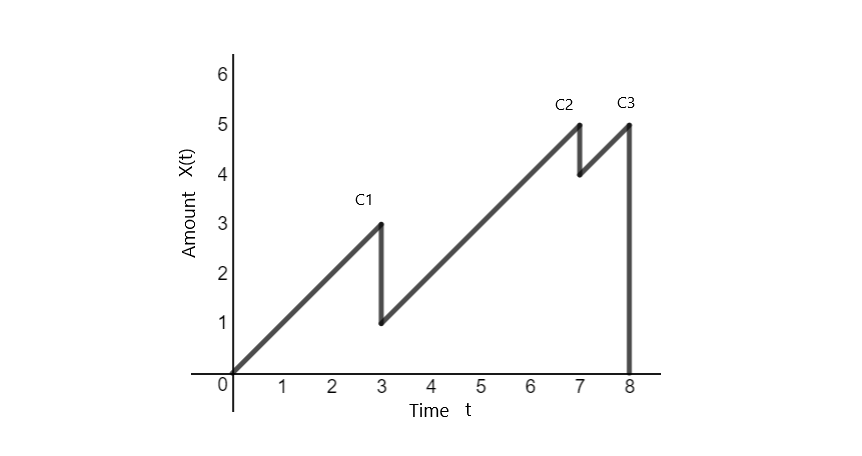
\includegraphics [width=3.3in]{CL1-1.png}
\end{center}
\end{figure}

We define the first passage times
\[ \tau_b^+ = \inf\{ t \geq 0, X(t) > b\}\]
\[ \tau_b^- = \inf\{ t \geq 0, X(t) < b\}\]
as the infimum values at which the process $X(t)$ goes above or below a certain value $b$.\\
Using this notation, we can denote the time of ruin as $\tau = \tau_0^-$. Moreover, if $X(t) > 0$ $\forall t\geq 0$, then we say $\tau = + \infty$.

Let $t, u >0$. The probability of ruin before time $t$ and given initial value $u$ is written as
\[\Psi(t|u) = \mathbb{P} [\tau < t | X(0)=u ].  \]
We refer to this scenario ruin in finite time.\\

Alternatively, one can study probabilities of survival in finite time by observing the function
\[ \bar {\Psi} (t|u) = \mathbb{P} [\tau \geq t | X(0)=u ] = 1 - \Psi (t|u) . \]

Letting the value of $t$ approach infinity, we get a quantity which can be interpreted as the probability of eventual ruin, or ruin in infinite time.

Let $u >0$. The probability of ruin given initial value $u$ is written as
\[\Psi(u) = \mathbb{P} [\tau < +\infty | X(0)=u ]. \]
Same as in the last definition, we also can study
\[ \bar {\Psi} (u) = \mathbb{P} [\tau = + \infty | X(0)=u ] = 1 - \Psi (u). \]

The \rp \ is a measure of the risk associated to a financial company.

For the case Cramer-Lundberg case, the following formula which may be inferred form the work of Pollaczek, Khinchine (\cite{Rolski}) was found great of great use in ruin theory (and in queueing theory) :
\[\hat \Psi(s) = \int_0^{\infty} e^{-s u} \Psi(u) du
= \frac{\lambda (m_1 - \hat{\bar{F}}(s))}{s (c-\lambda \hat{\bar{F}}(s)) }\]
where $\hat \Psi(s)$ and $\hat{\bar{F}}(s)$ are the Laplace transforms of the ruin function and the survival function of the claim distributions respectively, and $m_1$ is the first moment of the claims, which will be assumed from now on to be finite.

We state now several forms of this result,  emphasizing the relationship of $\hat \Psi(s)$ to the  crucial  Levy exponent $\kappa (s)$ of the underlying process. This is important, since results expressed in terms of $\kappa (s)$ hold typically for all \sn \lev \procs.

\begin{thm}[The Pollaczek-Khinchine formulas for the ruin function Laplace transform]
Let $X(t) = u + ct - S(t), \quad S(t) = \sum_{i=1}^{N_\lambda (t)} C_i$ be a Cram\'er Lundberg risk process and $\Psi$ its corresponding ruin function. Then the Laplace transforms of the ruin function and its corresponding survival function can be expressed as
\begin{align*}
\hat \Rui(s) &= \int_0^{\infty} e^{-s u} \Rui(u) du
= \frac{\lambda (m_1 - \hat{\bar{F}}(s))}{s (c-\lambda \hat{\bar{F}}(s)) } = \frac{1}{s}- \frac{ \kappa'(0)}{ \kappa(s)} \\
\hat \sRui(s) &= \int_0^{\infty} e^{-s u} \sRui(u) du = \frac{1}{s} - \hat \Rui(s) = \frac{\kappa'(0)}{\kappa(s)}.
\end{align*}
It is also possible to express this result in terms of 
the equilibrium density $f_e(x):=\bar{F}(x)/m_1$ and of $\rho =(\lambda m_1)/c$, since for Cramer Lundberg processes $\kappa(s) =  cs( 1- \rho \hat f_e(s)) $.
\end{thm}
\section{The Dividend Problem}

The notion of the problem of dividends is popularized by De Fenetti (\cite{deF}) and starts by considering a Cramer-Lundberg process $\{ X(t) \}_{t \in [0,\infty] }$ (we can of course consider more general cases) and another process $\{ L(t) \}_{t \in [0,\infty] }$ which is left continuous, nonnegative, and non decreasing.\\
\bigskip
The quantity $L(t)$ can be thought of as the cumulative dividends paid up to time $t$ of an insurance company and hence the risk process taking into account the dividends is $\{ U(t) \}_{t \in [0,\infty] }$ where
\[
U(t) = X(t) - L(t).
\]
The general problem is the characterization of $L$ and the maximization of $U$ through the choice of $L$, often called a dividend strategy.

A dividend strategy is called admissible if at any time before ruin, all dividend payments are smaller than the current value of $U$, that is
\[L(t^+) - L(t) \leq U(t), \quad \forall t < \tau\]
where $\tau$ is the ruin time of $U$.\\
\bigskip
There are a number of possible dividend strategies, hence one often associates another parameter to the process $L$, say $L^{\pi}$.

Denoting all admissible strategies by $\Pi$, we write the expected value at the discount rate $q\geq 0$ associated with the dividend strategy $\pi \in \Pi$ with initial surplus $x \geq 0$ as
\[
V^{\pi}(x) = \mbbE_x \lt[ \int_0^{\tau^{\pi}} e^{-qt} dL^{\pi}_t \rt].
\]
One may sometimes see $V^{\pi}$ being referred to as the value function associated with strategy $\pi$. The problem is the characterization of
\[
V(x) = \sup_{\pi \in \Pi} V^{\pi}(x).
\]

Under the barrier strategy studied by Avram (\cite{APP}), the  process $U$ is never allowed to go above a constant level $b>0$, by setting
\[ L(t) = (X(t)-a)^+ = \max \{0, X(t)-a\}. \]
That is, surplus above the barrier $b$ is always paid as dividend.

\begin{figure}
\begin{center}
\caption{Sample path for a risk process and under a dividend barrier $b$}
    \begin{subfigure}[b]{0.3\textwidth}
        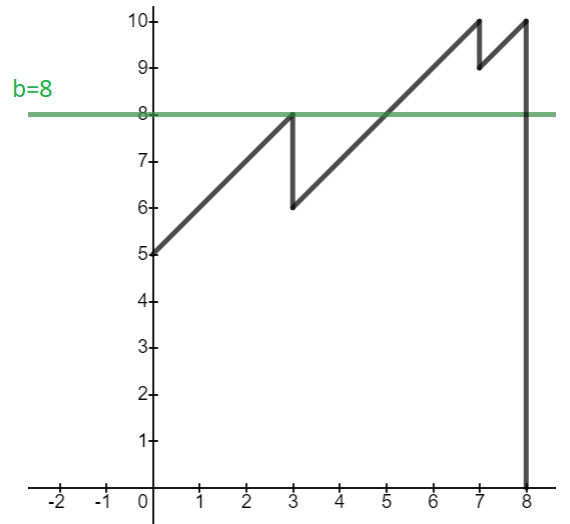
\includegraphics [width=2.2in]{divi1-1.png}
        \caption{$X(t)$}
        \label{fig:gull}
    \end{subfigure}\\
    \begin{subfigure}[b]{0.3\textwidth}
        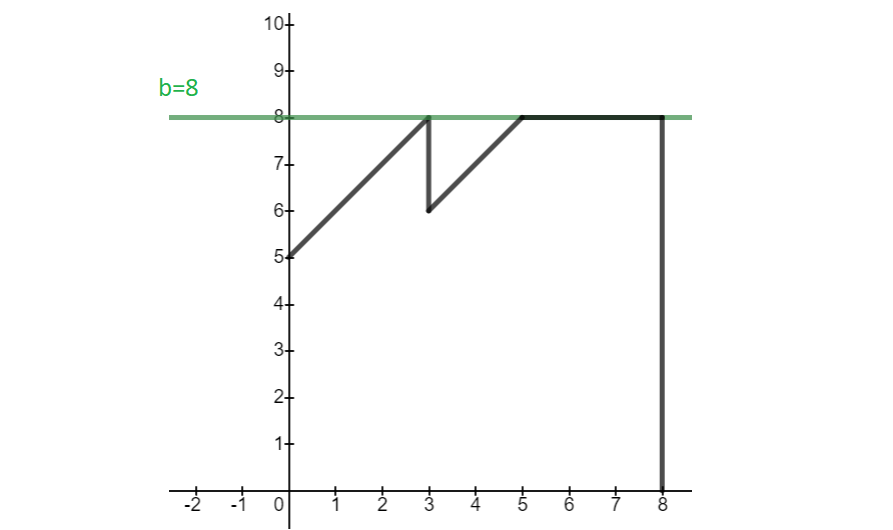
\includegraphics [width=3.3in]{divi2-1.png}
        \caption{$U(t)$}
        \label{fig:tiger}
    \end{subfigure}
\end{center}
\end{figure}

Clearly, this strategy, which we denote by $b] \in \Pi$, is admissible, and referencing Avram (2007), we have the following result.
\begin{thm}
Let $W_q$ be the associated scale function to $X$ under the discount rate $q\geq 0$. Under a constant dividend barrier strategy $b] \in \Pi$,
\[ V^{b]} (x) = \begin{cases}
\frac{W_q(x)}{W'_q(b)} & \text{ if $x \leq b$}\\
x - b + \frac{W_q(b)}{W'_q(b)} & \text{ if $x > b$}
\end{cases}
\]
\end{thm}

Looking at $V^{b]}$ as a function of $b$ instead of $x$, we can solve for $V$ by looking at where the derivative of $V^{b]}$ is zero. We summarize this result through the use of the `barrier function' $H$.
\begin{rmk}[\cite{APP}, \cite{Loef08}]
Let $b \geq 0$ and $H(b) = \frac{1}{W'_q (b)}$.\\
If $H$ is differentiable with $H'(0) > 0$, and has a unique local maximum $b^*>0$, then this $b^*$ yields the optimal barrier strategy, i.e. $V= V^{b^*]}$.\\
Furthermore, note that
\begin{itemize}
\item $H'(0) > 0 \iff W_q''(0)<0$
\item local maximum at $b^* \Rightarrow W_q''(b^*) =0$
\item uniqueness of local maximum at $b^* \Rightarrow H(b_1) \geq H(b_2)$, whenever $b* \leq b_1 \leq b_2$
\end{itemize}
\end{rmk}

This remark tells us that not only is $V^{b^*]}$ the optimal strategy over the space of the constant barrier strategies, but it is optimal over all strategies in $\Pi$.\\
\bigskip
We will not be tackling other dividend strategies in this presentation, nonetheless, we stress the fact that they do exist (see for example threshold strategies (\cite{gerber2004optimal}), multiband strategies (\cite{AM05}), etc.)

\subsection{The Cramer-Lundberg model with exponential jumps}
\label{CLexpo}

Consider the Cramer-Lundberg model $ X(t) = u + ct - S(t), \quad S(t) = \sum_{i=1}^{N_\lambda (t)} C_i $\\
where $C_i$'s are exponentially distributed with $\mbbE C_i = \frac{1}{\mu}$.\\
\bigskip
Standard computations yield
\[
\kappa(s)= s \lt( c- \frac{\lambda}{s + \mu} \rt), \quad \kappa'(0) = c - \frac{\lambda}{\mu}
\]
and solving
\[
\kappa(s)-q = 0 \iff cs^2 + (c\mu -\lambda -q ) s -q\mu = 0
\]
yields two distinct solutions $\gamma_1 \leq 0 \leq \gamma_2$ given by
\[
\gamma_1 = \frac{1}{2c} \lt( -(c\mu -\lambda -q ) + \sqrt{ (c\mu -\lambda -q )^2 + 4 c q\mu} \rt)
\]
\[
\gamma_1 = \frac{1}{2c} \lt( -(c\mu -\lambda -q ) - \sqrt{ (c\mu -\lambda -q )^2 + 4 c q\mu} \rt)
\]

In this example the Laplace transform of the $W_q$ scale function is
\[
\hat{W}_q(s) = \frac{1}{\kappa(s)-q} = \frac{s + \mu}{cs^2 + (c\mu -\lambda -q ) s -q\mu}
\]
which, when inverted becomes
\[
W_q(x) = \frac{(\gamma_1 + \mu)e^{\gamma_1 x} - (\gamma_2 + \mu) e^{\gamma_2 x} }{c(\gamma_1 - \gamma_2)}
\]

Differentiating we get
\[
W'_q(x) = \frac{\gamma_1(\gamma_1 + \mu)e^{\gamma_1 x} - \gamma_2(\gamma_2 + \mu) e^{\gamma_2 x} }{c(\gamma_1 - \gamma_2)}
\]
\[
W''_q(x) = \frac{\gamma_1^2(\gamma_1 + \mu)e^{\gamma_1 x} - \gamma_2^2(\gamma_2 + \mu) e^{\gamma_2 x} }{c(\gamma_1 - \gamma_2)}
\]
which implies
\[
W''_q(x) =0 \iff x = \frac{1}{\gamma_1 - \gamma_2} \log \frac{\gamma_2 (\gamma_2 + \mu)}{\gamma_1 (\gamma_1 + \mu)}.
\]

The function $W_q'(x)$ is unimodal with extremum at $x* = \frac{1}{\gamma_1 - \gamma_2} \log \frac{\gamma_2 (\gamma_2 + \mu)}{\gamma_1 (\gamma_1 + \mu)}$. Hence if
\[
W''_q(0)<0 \Rightarrow x* \text{ is a global minimum}
\]
and
\[
W''_q(0)\geq 0 \Rightarrow x* \text{ is a global maximum}.
\]
Therefore the optimal boundary $b*$ for the dividend problem is
\[
b*=
\begin{cases}
\frac{1}{\gamma_1 - \gamma_2} \log \frac{\gamma_2 (\gamma_2 + \mu)}{\gamma_1 (\gamma_1 + \mu)} & \text{ if } W''_q(0)<0\\
0 & \text{ if } W''_q(0)\geq 0.
\end{cases}
\]
\section{Approximations to the $W_q$ scale function}
Consider a spectrally negative Levy risk process $X = u + ct - S(t)$ and associated Levy measure $\nu$ with $\kappa(s) = s(c- \hat{\bar{\nu}} (s))$ as its Levy-Khintchine representation.\\

Letting $\nu_k = \int_{0}^{\infty} x^k \nu(dx)$ be the moments of the Levy measure. Then one can obtain a power series representation of the Levy exponent in terms of the moments given by
\[
\kappa(s) = s(c- \hat{\bar{\nu}} (s)) = cs + \sum_{k=1}^{\infty} \nu_k \frac{(-s)^k}{k!}.
\]
In the Cramer-Lundberg case where the intensity of the claim arrivals are given by the Poisson parameter $\lambda$, we have $\nu_k = \lambda m_k$ where $m_k$'s are the moments of the claims $C_i$.

One can thus write
\begin{align} \label{WMoments}
\hat{W}_q(s) = \frac{1}{\kappa(s)-q} =  \frac{1}{cs - \sum_{k=1}^{\infty} \nu_k \frac{(-s)^k}{k!} - q}.
\end{align}


\subsection{Pade Approximation}
\label{PadeApproxSection}
We can approximate (\ref{WMoments}) by a Pade approximation of order $[n-1,n]$
\begin{align}
\label{appxW}
\hat{W}_q(s) \approx \frac{P_{n-1}(s)}{Q_{n}(s)} = \frac{\sum_{i=0}^{n-1} a_i s^i}{cs^n + \sum_{i=0}^{n-1} b_i s^i}
\end{align}
for some polynomials $P_{n-1}$, $Q_n$, and some constants $a_i, b_i$, $i=0, \ldots, n-1$.

After the approximation the denominator can be factored as
\[
cs^n + \sum_{i=0}^{n-1} b_i s^i = c(s-\gamma_0) \prod_{i=1}^{n} (s+\gamma_i)
\]
and after a partial fraction decomposition of (\ref{appxW}) we get
\[
\hat{W}_q(s) \approx \frac{C_0}{s-\gamma_0} + \sum_{i=1}^{n} \frac{C_i}{s+\gamma_i}
\]
\[
\Rightarrow W_q(x) \approx C_0 e^{\gamma_0 x} + \sum_{i=1}^{n} C_i e^{-\gamma_i x}
\]

Looking back at the properties of the $W_q$ function in the Cramer-Lundberg case, we can force (\ref{W0}) and (\ref{Wprime0}) by setting $a_{n-1}=1$ and $ b_{n-1} = ca_{n-2} -\lambda - q$
\[
\hat{W}_q(s) \approx \frac{s^{n-1} + \sum_{i=0}^{n-2} a_i s^i}{cs^n + (c a_{n-2} -\lambda - q) s^{n-1} +\sum_{i=0}^{n-2} b_i s^i}.
\]

Since we are fitting two values $W_q(0)$ and $W'_q(0)$ into the Pade approximation, this would be a $[1,2]$ Pade approximant
\[
\hat{W}_q(s) \approx \frac{s + a_0}{cs^2 + (c a_0 -\lambda - q) s +b_0}.
\]

Comparing this with the true value of $\hat{W}_q(s)$,
\[
\hat{W}_q(s) = \frac{1}{\kappa(s)-q} \approx \frac{s + a_0}{cs^2 + (c a_0 -\lambda - q) s +b_0}
\]
\[
\Rightarrow cs^2 +(c a_0 -\lambda - q) s +b_0 \approx (s + a_0)(\kappa(s)-q)
\]
\[
\Rightarrow cs^2 +(c a_0 -\lambda - q) s +b_0 \approx (s + a_0)(cs -\nu_1 s +... -q)
\]
\[
\Rightarrow cs^2 +(c a_0 -\lambda - q) s +b_0 \approx (s + a_0)(cs -\lambda m_1 s  -q)
\]
\[
\Rightarrow a_0 = \frac{1}{m_1} \text{ and } b_0 = -\frac{q}{m_1}.
\]
That is,
\begin{align}
\label{WWprime}
\hat{W}_q(s) \approx \frac{s +  \frac{1}{m_1}}{cs^2 + ( \frac{c}{m_1} -\lambda - q) s -\frac{q}{m_1}}.
\end{align}

We note that the given approximation in (\ref{WWprime}) is the same approximation if we consider the claims to be exponential with $m_1 = \frac{1}{\mu}$, as in (\ref{CLexpo}).\\
\bigskip
The optimal boundary $b*$ for this approximation to the $W_q$ function is thus already been solved.

One can also approximate $W_q$ by a higher order Pade approximant, taking into account only (\ref{W0}).\\
That is, setting $n=2$ and $a_{n-1} = 1$ we have
\[
\hat{W}_q(s) = \frac{1}{\kappa(s)-q} \approx \frac{s + a_0}{cs^2 + b_1 s + b_0}.
\]
\[
\Rightarrow \hat{W}_q(s) \approx \frac{s + a_0}{cs^2 + b_1 s + b_0}.
\]
\[
\Rightarrow cs^2 +b_1 s +b_0 \approx (s + a_0)(\kappa(s)-q)
\]
\[
\Rightarrow cs^2 +b_1 s +b_0 \approx (s + a_0)(cs - \lambda m_1 s + \lambda m_2 \tfrac{s^2}{s} - q)
\]
\[
\Rightarrow a_0 = \frac{2m_1}{m_2}, b_1 = \frac{2c m_1 - 2\lambda m_1^2 - m_2 q}{m_2},
\]
\[
\text{ and } b_0 = -\frac{2m_1 q}{m_2}
\]

Therefore
\[
\hat{W}_q(s) \approx \frac{s +\frac{2m_1}{m_2}}{cs^2 + \lt( \frac{2c m_1 - 2\lambda m_1^2 - m_2 q}{m_2} \rt) s -\frac{2m_1 q}{m_2}}.
\]
This can be rewitten as
\[
\hat{W}_q(s) \approx \frac{s +\frac{1}{\tilde {m}_1}}{cs^2 + \lt( \frac{c}{\tilde{m}_1} - \lambda \frac{m_1}{\tilde{m}_1} -q \rt) s -\frac{q}{\tilde {m}_1}}.
\]
where $\tilde{m}_1 = \frac{m_2}{2m_1}$ is the first moment of the equilibrium density $f_e = \frac{\bar{F}}{m_1}$. This approximation is more commonly known as DeVylder's method (\cite{gerber2008methods}).

\subsection{Laguerre Approximation}
\label{LaguerreSec}
Consider the Laguerre polynomials
\[
L_n(x) = \frac{e^x}{n!} \cdot \frac{d^n}{dx^n}[e^{-x} x^n] = \sum_{k=0}^{n} \binom{n}{k} \frac{(-x)^k}{k!}
\]
for $x \geq 0$, $n=0, 1, \ldots$. These polynomials are orthogonal with respect to the weight $e^{-\frac{x}{2}}$, and for constant $\alpha$, $L_n(\alpha x)$ has Laplace transform given by
\[
\hat{L}_n(s) = \frac{(s-\alpha)^n}{s^{n+1}}, n=0,1, \ldots.
\]

Now, define $W^{(\Phi_q)}_0$ to be the $q=0$ scale function with respect to the Esscher transformed measure $P^{(\Phi_q)}$ (will not be discussed in detail, see (\cite{AA}), (\cite{Kyp})) given by
\[
W_q(x) = e^{x \Phi_q} \cdot W^{(\Phi_q)}_0 (x).
\]
By dividing by $e^{x \Phi_q}$, one removes the unique positive pole of $\hat{W}_q$
\[
\hat{W}_q(s) = \frac{1}{s - \Phi_q} \cdot \widehat{W^{(\Phi_q)}_0} (s)
\]
\[
\Rightarrow (s - \Phi_q)\hat{W}_q(s) = \widehat{W^{(\Phi_q)}_0} (s).
\]
By property of Laplace transforms we also know that
\begin{align*}
W^{(\Phi_q)}_0 (x) &=  e^{-x \Phi_q} \cdot W_q(x)\\
\Rightarrow \widehat{W^{(\Phi_q)}_0} (s) &= \hat{W}_q(s + \Phi_q) = \frac{1}{\kappa(s + \Phi_q) - q}\\
&= \frac{1}{\kappa(s + \Phi_q) - \kappa(\Phi_q)}.
\end{align*}

Following (\cite{abate1998numerical}), one can consider
\begin{align} \label{GW}
G(x) = W^{(\Phi_q)}_0(\infty) - W^{(\Phi_q)}_0 (x)
\end{align}
and approximate using Laguerre polynomials
\begin{align} \label{GB}
G(x) \approx C \sum_{n=0}^{\infty} B_n e^{-\alpha x/2} L_n(\alpha x)
\end{align}
for some chosen constants $C, \alpha$, and coefficients $B_n$ to be solved for. Taking the Laplace transform of (\ref{GW})
\begin{align}
\widehat{G (x)} = \widehat{W^{(\Phi_q)}_0(\infty)} - \widehat{W^{(\Phi_q)}_0 (x)} \nonumber \\
\hat{G}(s)= \frac{W^{(\Phi_q)}_0(\infty)}{s} - \widehat{W^{(\Phi_q)}_0} (s) \nonumber \\
=  \frac{W^{(\Phi_q)}_0(\infty)}{s} - \frac{1}{\kappa(s + \Phi_q) - \kappa(\Phi_q)}. \label{Hcomp1}
\end{align}
Taking the Laplace transform of (\ref{GB}) we have
\[
\hat{G}(s) \approx C \sum_{n=0}^{\infty} B_n \cdot \hat{L}_n(s+\alpha / 2) 
\]
\[
\hat{G}(s) \approx C \sum_{n=0}^{\infty} B_n \frac{(s - \alpha / 2)^n}{ (s+\alpha/2)^{n+1}}.
\]
Some computations yield
\begin{align}
\hat{H}(s) &= (s+\alpha/2) \hat{G}(s) \nonumber \\
& \approx C \sum_{n=0}^{\infty} B_n \frac{(s - \alpha / 2)^n}{ (s+\alpha/2)^{n}} \nonumber \\
\Rightarrow \hat{H} \lt( \frac{\alpha}{2} \cdot \frac{1+z}{1-z} \rt) &= \lt( \frac{\alpha}{1-z} \rt) \hat{G} \lt( \frac{\alpha}{2} \cdot \frac{1+z}{1-z} \rt) \label{Hcomp2} \\
&\approx C \sum_{n=0}^{\infty} B_n z^n \nonumber
\end{align}
upon using the `collocation' transformation $z = \frac{s - \alpha/2}{s + \alpha/2} \iff s = \frac{\alpha}{2} \cdot \frac{1+z}{1-z}$.

Hence we solve for the coefficients $B_n$ by taking the Taylor expansion of $\hat{H} \lt( \frac{\alpha}{2} \frac{1+z}{1-z} \rt)$ which is known to us via (\ref{Hcomp2}) and (\ref{Hcomp1}). The approximation we get for $G$ gives us an approximation for $ W^{(\Phi_q)}_0$. An approximation for $W_q$ is then obtained by multiplying by $e^{x \Phi_q}$.

With regards to the choice of $C$ and $\alpha$, one can do a first order Pade approximation discussed in (\ref{PadeApproxSection}), to obtain an approximation to $W^{(\Phi_q)}_0 (x)$ of the form
\[
W^{(\Phi_q)}_0 (x) \approx W^{(\Phi_q)}_0 (\infty) - C \frac{\alpha}{2} e^{-\frac{\alpha}{2}x}.
\]

\subsection{Example: a Cramer-Lundberg model with exponential mixture jumps of order two}
\label{exCL2}

Consider a Cramer-Lundberg process with $c=1/2$, $\lambda = 29/48$ with claim density given by $f(x) = \frac{8}{29}e^{-x} + \frac{42}{29} e^{-2x}$. To obtain rational values we fix $q=1/16$.

Computing the Levy exponent, one gets
\[
\kappa(s) = \frac{1}{2} s + \frac{8}{48} \lt( \frac{1}{s+1} - 1\rt) + \frac{21}{48} \lt( \frac{2}{s+2} -1 \rt)
\]
which then yields
\[
\hat{W}_q (s) = \frac{1}{\kappa(s) - 1/16} = \frac{24(s+1)(s+2)}{(3s-1)(2s+1)(2s+3)}
\]
\[
= -\frac{6}{11} \cdot \frac{1}{2s+3} - \frac{18}{5} \cdot \frac{1}{2s+1} +\frac{672}{55} \cdot \frac{1}{3s-1}
\]
\[
\Rightarrow W_q(x) = -\frac{3}{11} e^{-3x/2} - \frac{9}{5} e^{-x/2} +\frac{224}{55} e^{x/3}.
\]

\begin{figure}
\caption{Plot of $W_q^{''}$ in \ref{exCL2}}
\begin{center}
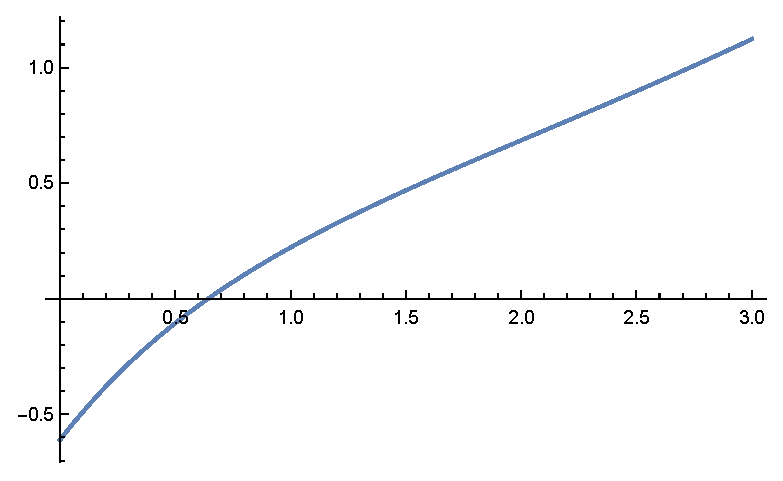
\includegraphics [width=2.8in]{pw2.eps}
\end{center}
\label{pw2}
\end{figure}

A plot of this scale function is given in (\ref{pw2}), and upon doing some calculations one gets the optimal barrier value $b^* = 0.642265$. Furthermore this reveals that the unique positive root $\Phi_q = 1/3$

Doing a Pade [2,3] approximation of $\hat{W}_q$ described in \ref{CLexpo} would yield the exact result (in fact, this is true for all Cramer Lundberg processes with mixed exponential claims of order 2).

Meanwhile, doing the approximation described in (\ref{LaguerreSec}), one first computes
\[
\widehat{W^{(\Phi_q)}_0 (x)} = \frac{8(3s+4)(3s+7)}{s(6s+5)(6s+11)}
\]
which then leads to
\[
\hat{G}(s) = \frac{72(57s+97)}{55(6s+5)(6s+11)}.
\]

\begin{figure}
\caption{Relative errors of the Laguerre approximation in \ref{exCL2}}
\begin{center}
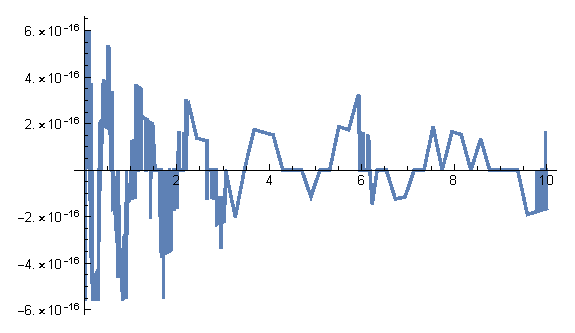
\includegraphics [width=2.8in]{err2.eps}
\end{center}
\label{err2}
\end{figure}

A [0,1] Pade approximation to $\hat{G}$ gives us $\frac{677448}{55(6177s + 5335)}$ implying the Laguerre exponent $\alpha/2 = 5335/6177 = 0.863688$. The resulting error in the Laguerre approximation is plotted in (\ref{err2}), with the largest error being $6*10^{-6}$ when 30 terms are considered in the Laguerre expansion.



\section{The $W_q$ scale function and Discounting}
The underlying structure of ruin theory appears more clearly after generalizing the ruin problem to the two sided exit problem. Assume $a<b$, and consider quantities such as $\tau_a^+$, $\tau_b^-$, $\tau := \min\{ \tau_a^+, \tau_b^- \}$ and
\[ \Rui_{a,b}(x) = \mathbb{P}_x [\tau_a^+ < \tau_b^-] \]
\[ \sRui_{a,b}(x) = \mathbb{P}_x [\tau_a^+ > \tau_b^-]. \]

\begin{figure}
\caption{Sample path for a two sided exit problem}
\begin{center}
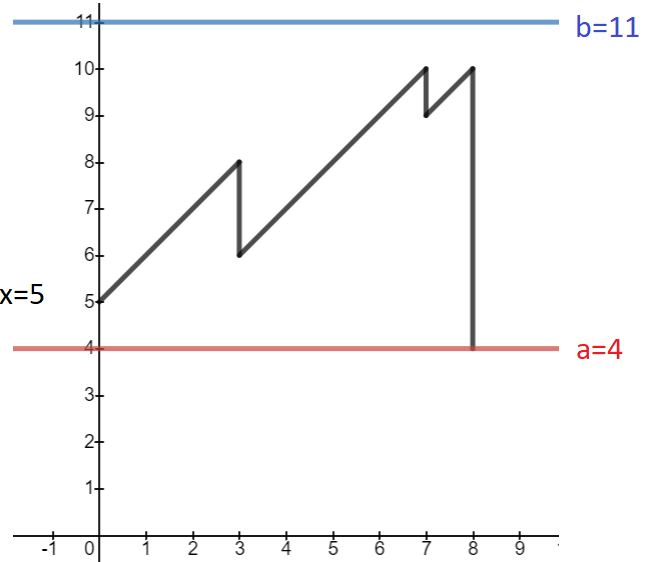
\includegraphics [width=2.3in]{twosided2.png}
\end{center}
\end{figure}

It can be shown, via the Markov property of the underlying process, that for some function $W$, we have
\[ \sRui_{a,b}(x) = \frac{W(x-a)}{W(b-a)}\]
We will refer to this function $W$ (determined up to a proportionality constant) as the $W$ scale function of the process.
Furthermore upon taking the Laplace transform of the previous equation we get
\[ \hat \sRui_{a,b}(s) = \frac{\hat W(s)}{W(b-a)}, \]
and in the case of the ruin problem where $\hat \sRui(s) = \frac{\kappa'(0)}{\kappa(s)}$, we get the idea that \[\hat W(s) = C \frac{1}{\kappa(s)}\] up to a certain constant $C$.

Generalizing further, suppose there exist an `interest rate' $q \geq 0$ such that one considers the `discounted value' of the underlying process with respect to this $q$ when deciding for the  first passage time.\\
In this scenario,
\[ \sRui_{a,b}(x) = \mathbb{E}_x [ e^{-q \tau_b^+} \cdot \mathbbm{1}_{\{\tau_a^+ > \tau_b^-\}}] \]
where $\mathbbm{1}_{A}$ is the event that $A$ happens.\\
Here the probability of survival considers all events where $\tau_a^+ > \tau_b^-$, and gets the expected value of the discounted value of 1 at the time $\tau_b^+$ with respect to $q$, hence the term $e^{-q \tau_b^+}$.

Even with discounting, through the same analysis as before one can find a function $W_q$ for which
\[ \sRui_{a,b}(x) = \frac{W_q(x-a)}{W_q(b-a)}. \]
In fact if one defines $W_q(s): (0,+\infty) \rightarrow [0,+\infty)$ to have a Laplace transform
\[ \hat{W}_q(s) = \int_0^{\infty} e^{-sx} W_q(x) ~dx  := \frac{1}{\kappa(s) - q} \quad \forall s > \Phi (q), \]
where $\Phi (q) := \sup \{ s\geq 0 : \kappa(s) - q = 0 \}$, one would arrive at such a function. As before we call this the $W_q$ scale function of the underlying process.\\

\begin{rmk} [\cite{Bingham}, \cite{Ber}, \cite{Kyp}]
The scale function $W_q$ is continuous and increasing on $[0,\infty]$.
\end{rmk}

\begin{rmk} [\cite{Kyprianou_Surya},\cite{KKP}]
The behavior in the neighborhood of zero of $W_q$ can be obtained from the behavior of its Laplace transform $\hat{W}_q$ at $\infty$
\begin{align}
\label{W0}
W_q (0^+) &= \lim_{s\rightarrow \infty} \frac{s}{\kappa(s)-q}= \begin{cases} \frac{1}{c} &\text{ if $X$ is of bdd variation}\\ 0 &
\text{ if $X$ is of unbdd variation} \end{cases}\\
\nonumber  W'_q (0^+) &= \lim_{s\rightarrow \infty} s\lt( \frac{s}{\kappa(s)-q} - W_q(0) \rt) \\
\label{Wprime0} &= \begin{cases} \frac{q + \nu (u,\infty)}{c^2} &\text{ if $X$ is of bdd variation}\\ \frac{2}{\sigma^2} & \text{ if $X$ is of unbdd variation} \end{cases}
\end{align}
\end{rmk}

\section{Minimizing the ruin probability via reinsurance}
Of course, insurance (and  reinsurance) are not for free; they influence the  premium income of the  insurers  via so called premium principles.

{\bf Premium principles} are specified by a deterministic
premium function $\pi : L_1 (\Omega, P) \to [0,\I)$. Some of the most popular choices are

a) the \textit{expectation principle},   with
$$\pi (Z) = (1 + \eta)E[Z],$$
where $\eta $ denotes a safety loading %of the reinsurer,

b) the \textit{variance principle}
$$\pi (Z) = E[Z] + \eta Var [Z]$$ %for $\a Var [Y] > \th m_1$.

c) the \textit{exponential principle}
$$\pi (Z) = \frac{E[e^{\eta Z}]-1}{\eta}.$$

Under the assumption of the expected
value principle, \ith:
\bea c=(1+\th) E \sum_{i=1}^{N_\l(1)} C_i=(1+\th) \l m_1,\eea
where $\th > 0$ is the safety loading for the insurer. 

Suppose now that the insurer attempts to reduce his risk exposure by purchasing a proportional reinsurance
with a retention level of $\a \in [0, 1]$. Specifically, for each claim of size $C_i$, the insurer covers $\a C_i$ and the reinsurer
covers the rest $(1-\a) C_i$.
 Suppose that the reinsurer also uses the expected premium principle, but with a larger
safety loading $\eta >\th$ (the reinsurance is then called ``non-cheap").  The premium rate for reinsurance is then
\bea c_\a =(1+\eta) (1-\a)\l m_1.\eea
Then, the surplus process with reinsurance can be expressed as
\begin{eqnarray*} \la{CLr}
\T X^{(\a)}_t &=& x + (c-c_\a) t  - \a \sum_{i=1}^{N_\lambda (t)} C_i\\&=& x + \l m_1\Big( \th -\eta+ \a(1+\eta)\Big) t  - \a \sum_{i=1}^{N_\lambda (t)} C_i.
\end{eqnarray*}

The underlying question is how to chose $\a$ in order to minimize the probability of ruin.


\bibliographystyle{plainnat}
\bibliography{Pare36}

%----------------------------------------------------------------------------------------

\end{document}
